% Created by tikzDevice version 0.12 on 2018-10-06 03:06:08
% !TEX encoding = UTF-8 Unicode
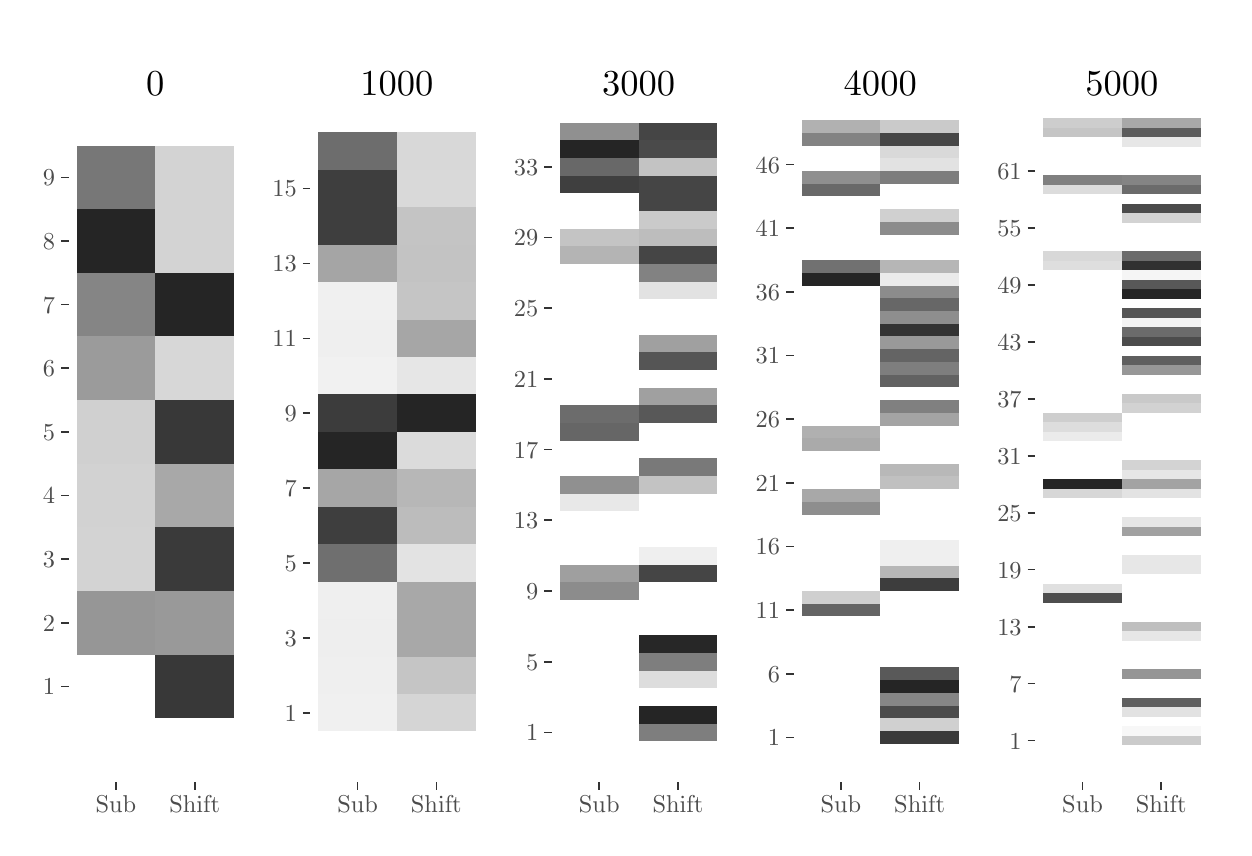
\begin{tikzpicture}[x=1pt,y=1pt]
\definecolor{fillColor}{RGB}{255,255,255}
\path[use as bounding box,fill=fillColor,fill opacity=0.00] (0,0) rectangle (432.17,289.08);
\begin{scope}
\path[clip] (  0.00,  0.00) rectangle ( 82.92,289.08);
\definecolor{drawColor}{RGB}{255,255,255}
\definecolor{fillColor}{RGB}{255,255,255}

\path[draw=drawColor,line width= 0.6pt,line join=round,line cap=round,fill=fillColor] (  0.00,  0.00) rectangle ( 82.92,289.08);
\end{scope}
\begin{scope}
\path[clip] ( 82.92,  0.00) rectangle (170.23,289.08);
\definecolor{drawColor}{RGB}{255,255,255}
\definecolor{fillColor}{RGB}{255,255,255}

\path[draw=drawColor,line width= 0.6pt,line join=round,line cap=round,fill=fillColor] ( 82.92,  0.00) rectangle (170.23,289.08);
\end{scope}
\begin{scope}
\path[clip] (170.23,  0.00) rectangle (257.55,289.08);
\definecolor{drawColor}{RGB}{255,255,255}
\definecolor{fillColor}{RGB}{255,255,255}

\path[draw=drawColor,line width= 0.6pt,line join=round,line cap=round,fill=fillColor] (170.23,  0.00) rectangle (257.55,289.08);
\end{scope}
\begin{scope}
\path[clip] (257.55,  0.00) rectangle (344.86,289.08);
\definecolor{drawColor}{RGB}{255,255,255}
\definecolor{fillColor}{RGB}{255,255,255}

\path[draw=drawColor,line width= 0.6pt,line join=round,line cap=round,fill=fillColor] (257.55,  0.00) rectangle (344.86,289.08);
\end{scope}
\begin{scope}
\path[clip] (344.86,  0.00) rectangle (432.17,289.08);
\definecolor{drawColor}{RGB}{255,255,255}
\definecolor{fillColor}{RGB}{255,255,255}

\path[draw=drawColor,line width= 0.6pt,line join=round,line cap=round,fill=fillColor] (344.86,  0.00) rectangle (432.17,289.08);
\end{scope}
\begin{scope}
\path[clip] ( 14.85, 16.51) rectangle ( 77.42,269.49);
\definecolor{drawColor}{RGB}{255,255,255}

\path[draw=drawColor,line width= 0.3pt,line join=round] ( 14.85, 28.01) --
	( 77.42, 28.01);

\path[draw=drawColor,line width= 0.3pt,line join=round] ( 14.85, 39.51) --
	( 77.42, 39.51);

\path[draw=drawColor,line width= 0.3pt,line join=round] ( 14.85, 62.51) --
	( 77.42, 62.51);

\path[draw=drawColor,line width= 0.3pt,line join=round] ( 14.85, 85.50) --
	( 77.42, 85.50);

\path[draw=drawColor,line width= 0.3pt,line join=round] ( 14.85,108.50) --
	( 77.42,108.50);

\path[draw=drawColor,line width= 0.3pt,line join=round] ( 14.85,131.50) --
	( 77.42,131.50);

\path[draw=drawColor,line width= 0.3pt,line join=round] ( 14.85,154.50) --
	( 77.42,154.50);

\path[draw=drawColor,line width= 0.3pt,line join=round] ( 14.85,177.50) --
	( 77.42,177.50);

\path[draw=drawColor,line width= 0.3pt,line join=round] ( 14.85,200.49) --
	( 77.42,200.49);

\path[draw=drawColor,line width= 0.3pt,line join=round] ( 14.85,223.49) --
	( 77.42,223.49);

\path[draw=drawColor,line width= 0.3pt,line join=round] ( 14.85,246.49) --
	( 77.42,246.49);

\path[draw=drawColor,line width= 0.3pt,line join=round] ( 14.85,257.99) --
	( 77.42,257.99);

\path[draw=drawColor,line width= 0.6pt,line join=round] ( 14.85, 51.01) --
	( 77.42, 51.01);

\path[draw=drawColor,line width= 0.6pt,line join=round] ( 14.85, 74.01) --
	( 77.42, 74.01);

\path[draw=drawColor,line width= 0.6pt,line join=round] ( 14.85, 97.00) --
	( 77.42, 97.00);

\path[draw=drawColor,line width= 0.6pt,line join=round] ( 14.85,120.00) --
	( 77.42,120.00);

\path[draw=drawColor,line width= 0.6pt,line join=round] ( 14.85,143.00) --
	( 77.42,143.00);

\path[draw=drawColor,line width= 0.6pt,line join=round] ( 14.85,166.00) --
	( 77.42,166.00);

\path[draw=drawColor,line width= 0.6pt,line join=round] ( 14.85,189.00) --
	( 77.42,189.00);

\path[draw=drawColor,line width= 0.6pt,line join=round] ( 14.85,211.99) --
	( 77.42,211.99);

\path[draw=drawColor,line width= 0.6pt,line join=round] ( 14.85,234.99) --
	( 77.42,234.99);

\path[draw=drawColor,line width= 0.6pt,line join=round] ( 31.91, 16.51) --
	( 31.91,269.49);

\path[draw=drawColor,line width= 0.6pt,line join=round] ( 60.35, 16.51) --
	( 60.35,269.49);
\definecolor{fillColor}{RGB}{255,255,255}

\path[fill=fillColor] ( 17.69, 39.51) rectangle ( 46.13, 62.51);
\definecolor{fillColor}{gray}{0.59}

\path[fill=fillColor] ( 17.69, 62.51) rectangle ( 46.13, 85.50);
\definecolor{fillColor}{RGB}{211,211,211}

\path[fill=fillColor] ( 17.69, 85.50) rectangle ( 46.13,108.50);
\definecolor{fillColor}{RGB}{210,210,210}

\path[fill=fillColor] ( 17.69,108.50) rectangle ( 46.13,131.50);
\definecolor{fillColor}{RGB}{208,208,208}

\path[fill=fillColor] ( 17.69,131.50) rectangle ( 46.13,154.50);
\definecolor{fillColor}{RGB}{155,155,155}

\path[fill=fillColor] ( 17.69,154.50) rectangle ( 46.13,177.50);
\definecolor{fillColor}{gray}{0.52}

\path[fill=fillColor] ( 17.69,177.50) rectangle ( 46.13,200.49);
\definecolor{fillColor}{RGB}{37,37,37}

\path[fill=fillColor] ( 17.69,200.49) rectangle ( 46.13,223.49);
\definecolor{fillColor}{RGB}{119,119,119}

\path[fill=fillColor] ( 17.69,223.49) rectangle ( 46.13,246.49);
\definecolor{fillColor}{gray}{0.22}

\path[fill=fillColor] ( 46.13, 39.51) rectangle ( 74.57, 62.51);
\definecolor{fillColor}{gray}{0.60}

\path[fill=fillColor] ( 46.13, 62.51) rectangle ( 74.57, 85.50);
\definecolor{fillColor}{RGB}{58,58,58}

\path[fill=fillColor] ( 46.13, 85.50) rectangle ( 74.57,108.50);
\definecolor{fillColor}{gray}{0.66}

\path[fill=fillColor] ( 46.13,108.50) rectangle ( 74.57,131.50);
\definecolor{fillColor}{gray}{0.22}

\path[fill=fillColor] ( 46.13,131.50) rectangle ( 74.57,154.50);
\definecolor{fillColor}{RGB}{215,215,215}

\path[fill=fillColor] ( 46.13,154.50) rectangle ( 74.57,177.50);
\definecolor{fillColor}{RGB}{37,37,37}

\path[fill=fillColor] ( 46.13,177.50) rectangle ( 74.57,200.49);
\definecolor{fillColor}{RGB}{211,211,211}

\path[fill=fillColor] ( 46.13,200.49) rectangle ( 74.57,223.49);

\path[fill=fillColor] ( 46.13,223.49) rectangle ( 74.57,246.49);
\end{scope}
\begin{scope}
\path[clip] (102.16, 16.51) rectangle (164.73,269.49);
\definecolor{drawColor}{RGB}{255,255,255}

\path[draw=drawColor,line width= 0.3pt,line join=round] (102.16, 28.01) --
	(164.73, 28.01);

\path[draw=drawColor,line width= 0.3pt,line join=round] (102.16, 55.07) --
	(164.73, 55.07);

\path[draw=drawColor,line width= 0.3pt,line join=round] (102.16, 82.12) --
	(164.73, 82.12);

\path[draw=drawColor,line width= 0.3pt,line join=round] (102.16,109.18) --
	(164.73,109.18);

\path[draw=drawColor,line width= 0.3pt,line join=round] (102.16,136.24) --
	(164.73,136.24);

\path[draw=drawColor,line width= 0.3pt,line join=round] (102.16,163.29) --
	(164.73,163.29);

\path[draw=drawColor,line width= 0.3pt,line join=round] (102.16,190.35) --
	(164.73,190.35);

\path[draw=drawColor,line width= 0.3pt,line join=round] (102.16,217.41) --
	(164.73,217.41);

\path[draw=drawColor,line width= 0.3pt,line join=round] (102.16,244.46) --
	(164.73,244.46);

\path[draw=drawColor,line width= 0.3pt,line join=round] (102.16,257.99) --
	(164.73,257.99);

\path[draw=drawColor,line width= 0.6pt,line join=round] (102.16, 41.54) --
	(164.73, 41.54);

\path[draw=drawColor,line width= 0.6pt,line join=round] (102.16, 68.59) --
	(164.73, 68.59);

\path[draw=drawColor,line width= 0.6pt,line join=round] (102.16, 95.65) --
	(164.73, 95.65);

\path[draw=drawColor,line width= 0.6pt,line join=round] (102.16,122.71) --
	(164.73,122.71);

\path[draw=drawColor,line width= 0.6pt,line join=round] (102.16,149.76) --
	(164.73,149.76);

\path[draw=drawColor,line width= 0.6pt,line join=round] (102.16,176.82) --
	(164.73,176.82);

\path[draw=drawColor,line width= 0.6pt,line join=round] (102.16,203.88) --
	(164.73,203.88);

\path[draw=drawColor,line width= 0.6pt,line join=round] (102.16,230.93) --
	(164.73,230.93);

\path[draw=drawColor,line width= 0.6pt,line join=round] (119.23, 16.51) --
	(119.23,269.49);

\path[draw=drawColor,line width= 0.6pt,line join=round] (147.67, 16.51) --
	(147.67,269.49);
\definecolor{fillColor}{gray}{0.94}

\path[fill=fillColor] (105.01, 34.77) rectangle (133.45, 48.30);
\definecolor{fillColor}{RGB}{239,239,239}

\path[fill=fillColor] (105.01, 48.30) rectangle (133.45, 61.83);
\definecolor{fillColor}{RGB}{238,238,238}

\path[fill=fillColor] (105.01, 61.83) rectangle (133.45, 75.36);
\definecolor{fillColor}{RGB}{239,239,239}

\path[fill=fillColor] (105.01, 75.36) rectangle (133.45, 88.89);
\definecolor{fillColor}{RGB}{111,111,111}

\path[fill=fillColor] (105.01, 88.89) rectangle (133.45,102.42);
\definecolor{fillColor}{RGB}{62,62,62}

\path[fill=fillColor] (105.01,102.42) rectangle (133.45,115.94);
\definecolor{fillColor}{gray}{0.65}

\path[fill=fillColor] (105.01,115.94) rectangle (133.45,129.47);
\definecolor{fillColor}{RGB}{37,37,37}

\path[fill=fillColor] (105.01,129.47) rectangle (133.45,143.00);
\definecolor{fillColor}{RGB}{60,60,60}

\path[fill=fillColor] (105.01,143.00) rectangle (133.45,156.53);
\definecolor{fillColor}{RGB}{241,241,241}

\path[fill=fillColor] (105.01,156.53) rectangle (133.45,170.06);
\definecolor{fillColor}{RGB}{239,239,239}

\path[fill=fillColor] (105.01,170.06) rectangle (133.45,183.58);
\definecolor{fillColor}{gray}{0.94}

\path[fill=fillColor] (105.01,183.58) rectangle (133.45,197.11);
\definecolor{fillColor}{RGB}{165,165,165}

\path[fill=fillColor] (105.01,197.11) rectangle (133.45,210.64);
\definecolor{fillColor}{RGB}{62,62,62}

\path[fill=fillColor] (105.01,210.64) rectangle (133.45,224.17);

\path[fill=fillColor] (105.01,224.17) rectangle (133.45,237.70);
\definecolor{fillColor}{RGB}{109,109,109}

\path[fill=fillColor] (105.01,237.70) rectangle (133.45,251.23);
\definecolor{fillColor}{RGB}{213,213,213}

\path[fill=fillColor] (133.45, 34.77) rectangle (161.89, 48.30);
\definecolor{fillColor}{RGB}{197,197,197}

\path[fill=fillColor] (133.45, 48.30) rectangle (161.89, 61.83);
\definecolor{fillColor}{gray}{0.66}

\path[fill=fillColor] (133.45, 61.83) rectangle (161.89, 75.36);

\path[fill=fillColor] (133.45, 75.36) rectangle (161.89, 88.89);
\definecolor{fillColor}{gray}{0.89}

\path[fill=fillColor] (133.45, 88.89) rectangle (161.89,102.42);
\definecolor{fillColor}{RGB}{188,188,188}

\path[fill=fillColor] (133.45,102.42) rectangle (161.89,115.94);
\definecolor{fillColor}{RGB}{183,183,183}

\path[fill=fillColor] (133.45,115.94) rectangle (161.89,129.47);
\definecolor{fillColor}{gray}{0.86}

\path[fill=fillColor] (133.45,129.47) rectangle (161.89,143.00);
\definecolor{fillColor}{RGB}{37,37,37}

\path[fill=fillColor] (133.45,143.00) rectangle (161.89,156.53);
\definecolor{fillColor}{RGB}{230,230,230}

\path[fill=fillColor] (133.45,156.53) rectangle (161.89,170.06);
\definecolor{fillColor}{gray}{0.65}

\path[fill=fillColor] (133.45,170.06) rectangle (161.89,183.58);
\definecolor{fillColor}{RGB}{197,197,197}

\path[fill=fillColor] (133.45,183.58) rectangle (161.89,197.11);
\definecolor{fillColor}{RGB}{195,195,195}

\path[fill=fillColor] (133.45,197.11) rectangle (161.89,210.64);
\definecolor{fillColor}{gray}{0.77}

\path[fill=fillColor] (133.45,210.64) rectangle (161.89,224.17);
\definecolor{fillColor}{gray}{0.85}

\path[fill=fillColor] (133.45,224.17) rectangle (161.89,237.70);
\definecolor{fillColor}{RGB}{216,216,216}

\path[fill=fillColor] (133.45,237.70) rectangle (161.89,251.23);
\end{scope}
\begin{scope}
\path[clip] (189.48, 16.51) rectangle (252.05,269.49);
\definecolor{drawColor}{RGB}{255,255,255}

\path[draw=drawColor,line width= 0.3pt,line join=round] (189.48, 21.62) --
	(252.05, 21.62);

\path[draw=drawColor,line width= 0.3pt,line join=round] (189.48, 47.17) --
	(252.05, 47.17);

\path[draw=drawColor,line width= 0.3pt,line join=round] (189.48, 72.73) --
	(252.05, 72.73);

\path[draw=drawColor,line width= 0.3pt,line join=round] (189.48, 98.28) --
	(252.05, 98.28);

\path[draw=drawColor,line width= 0.3pt,line join=round] (189.48,123.83) --
	(252.05,123.83);

\path[draw=drawColor,line width= 0.3pt,line join=round] (189.48,149.39) --
	(252.05,149.39);

\path[draw=drawColor,line width= 0.3pt,line join=round] (189.48,174.94) --
	(252.05,174.94);

\path[draw=drawColor,line width= 0.3pt,line join=round] (189.48,200.49) --
	(252.05,200.49);

\path[draw=drawColor,line width= 0.3pt,line join=round] (189.48,226.05) --
	(252.05,226.05);

\path[draw=drawColor,line width= 0.3pt,line join=round] (189.48,251.60) --
	(252.05,251.60);

\path[draw=drawColor,line width= 0.3pt,line join=round] (189.48,264.38) --
	(252.05,264.38);

\path[draw=drawColor,line width= 0.6pt,line join=round] (189.48, 34.40) --
	(252.05, 34.40);

\path[draw=drawColor,line width= 0.6pt,line join=round] (189.48, 59.95) --
	(252.05, 59.95);

\path[draw=drawColor,line width= 0.6pt,line join=round] (189.48, 85.50) --
	(252.05, 85.50);

\path[draw=drawColor,line width= 0.6pt,line join=round] (189.48,111.06) --
	(252.05,111.06);

\path[draw=drawColor,line width= 0.6pt,line join=round] (189.48,136.61) --
	(252.05,136.61);

\path[draw=drawColor,line width= 0.6pt,line join=round] (189.48,162.16) --
	(252.05,162.16);

\path[draw=drawColor,line width= 0.6pt,line join=round] (189.48,187.72) --
	(252.05,187.72);

\path[draw=drawColor,line width= 0.6pt,line join=round] (189.48,213.27) --
	(252.05,213.27);

\path[draw=drawColor,line width= 0.6pt,line join=round] (189.48,238.82) --
	(252.05,238.82);

\path[draw=drawColor,line width= 0.6pt,line join=round] (206.54, 16.51) --
	(206.54,269.49);

\path[draw=drawColor,line width= 0.6pt,line join=round] (234.98, 16.51) --
	(234.98,269.49);
\definecolor{fillColor}{RGB}{255,255,255}

\path[fill=fillColor] (192.32, 31.20) rectangle (220.76, 37.59);

\path[fill=fillColor] (192.32, 37.59) rectangle (220.76, 43.98);

\path[fill=fillColor] (192.32, 43.98) rectangle (220.76, 50.37);

\path[fill=fillColor] (192.32, 50.37) rectangle (220.76, 56.76);

\path[fill=fillColor] (192.32, 56.76) rectangle (220.76, 63.15);

\path[fill=fillColor] (192.32, 63.15) rectangle (220.76, 69.53);

\path[fill=fillColor] (192.32, 69.53) rectangle (220.76, 75.92);

\path[fill=fillColor] (192.32, 75.92) rectangle (220.76, 82.31);
\definecolor{fillColor}{gray}{0.55}

\path[fill=fillColor] (192.32, 82.31) rectangle (220.76, 88.70);
\definecolor{fillColor}{RGB}{159,159,159}

\path[fill=fillColor] (192.32, 88.70) rectangle (220.76, 95.09);
\definecolor{fillColor}{RGB}{255,255,255}

\path[fill=fillColor] (192.32, 95.09) rectangle (220.76,101.48);

\path[fill=fillColor] (192.32,101.48) rectangle (220.76,107.86);

\path[fill=fillColor] (192.32,107.86) rectangle (220.76,114.25);
\definecolor{fillColor}{gray}{0.91}

\path[fill=fillColor] (192.32,114.25) rectangle (220.76,120.64);
\definecolor{fillColor}{RGB}{144,144,144}

\path[fill=fillColor] (192.32,120.64) rectangle (220.76,127.03);
\definecolor{fillColor}{RGB}{255,255,255}

\path[fill=fillColor] (192.32,127.03) rectangle (220.76,133.42);

\path[fill=fillColor] (192.32,133.42) rectangle (220.76,139.81);
\definecolor{fillColor}{gray}{0.40}

\path[fill=fillColor] (192.32,139.81) rectangle (220.76,146.19);
\definecolor{fillColor}{RGB}{108,108,108}

\path[fill=fillColor] (192.32,146.19) rectangle (220.76,152.58);
\definecolor{fillColor}{RGB}{255,255,255}

\path[fill=fillColor] (192.32,152.58) rectangle (220.76,158.97);

\path[fill=fillColor] (192.32,158.97) rectangle (220.76,165.36);

\path[fill=fillColor] (192.32,165.36) rectangle (220.76,171.75);

\path[fill=fillColor] (192.32,171.75) rectangle (220.76,178.14);

\path[fill=fillColor] (192.32,178.14) rectangle (220.76,184.52);

\path[fill=fillColor] (192.32,184.52) rectangle (220.76,190.91);

\path[fill=fillColor] (192.32,190.91) rectangle (220.76,197.30);

\path[fill=fillColor] (192.32,197.30) rectangle (220.76,203.69);
\definecolor{fillColor}{RGB}{180,180,180}

\path[fill=fillColor] (192.32,203.69) rectangle (220.76,210.08);
\definecolor{fillColor}{gray}{0.77}

\path[fill=fillColor] (192.32,210.08) rectangle (220.76,216.47);
\definecolor{fillColor}{RGB}{255,255,255}

\path[fill=fillColor] (192.32,216.47) rectangle (220.76,222.85);

\path[fill=fillColor] (192.32,222.85) rectangle (220.76,229.24);
\definecolor{fillColor}{RGB}{63,63,63}

\path[fill=fillColor] (192.32,229.24) rectangle (220.76,235.63);
\definecolor{fillColor}{RGB}{104,104,104}

\path[fill=fillColor] (192.32,235.63) rectangle (220.76,242.02);
\definecolor{fillColor}{RGB}{37,37,37}

\path[fill=fillColor] (192.32,242.02) rectangle (220.76,248.41);
\definecolor{fillColor}{RGB}{144,144,144}

\path[fill=fillColor] (192.32,248.41) rectangle (220.76,254.80);
\definecolor{fillColor}{RGB}{126,126,126}

\path[fill=fillColor] (220.76, 31.20) rectangle (249.20, 37.59);
\definecolor{fillColor}{RGB}{37,37,37}

\path[fill=fillColor] (220.76, 37.59) rectangle (249.20, 43.98);
\definecolor{fillColor}{RGB}{255,255,255}

\path[fill=fillColor] (220.76, 43.98) rectangle (249.20, 50.37);
\definecolor{fillColor}{RGB}{221,221,221}

\path[fill=fillColor] (220.76, 50.37) rectangle (249.20, 56.76);
\definecolor{fillColor}{RGB}{126,126,126}

\path[fill=fillColor] (220.76, 56.76) rectangle (249.20, 63.15);
\definecolor{fillColor}{RGB}{39,39,39}

\path[fill=fillColor] (220.76, 63.15) rectangle (249.20, 69.53);
\definecolor{fillColor}{RGB}{255,255,255}

\path[fill=fillColor] (220.76, 69.53) rectangle (249.20, 75.92);

\path[fill=fillColor] (220.76, 75.92) rectangle (249.20, 82.31);

\path[fill=fillColor] (220.76, 82.31) rectangle (249.20, 88.70);
\definecolor{fillColor}{gray}{0.27}

\path[fill=fillColor] (220.76, 88.70) rectangle (249.20, 95.09);
\definecolor{fillColor}{RGB}{239,239,239}

\path[fill=fillColor] (220.76, 95.09) rectangle (249.20,101.48);
\definecolor{fillColor}{RGB}{255,255,255}

\path[fill=fillColor] (220.76,101.48) rectangle (249.20,107.86);

\path[fill=fillColor] (220.76,107.86) rectangle (249.20,114.25);

\path[fill=fillColor] (220.76,114.25) rectangle (249.20,120.64);
\definecolor{fillColor}{RGB}{195,195,195}

\path[fill=fillColor] (220.76,120.64) rectangle (249.20,127.03);
\definecolor{fillColor}{RGB}{121,121,121}

\path[fill=fillColor] (220.76,127.03) rectangle (249.20,133.42);
\definecolor{fillColor}{RGB}{255,255,255}

\path[fill=fillColor] (220.76,133.42) rectangle (249.20,139.81);

\path[fill=fillColor] (220.76,139.81) rectangle (249.20,146.19);
\definecolor{fillColor}{RGB}{88,88,88}

\path[fill=fillColor] (220.76,146.19) rectangle (249.20,152.58);
\definecolor{fillColor}{RGB}{160,160,160}

\path[fill=fillColor] (220.76,152.58) rectangle (249.20,158.97);
\definecolor{fillColor}{RGB}{255,255,255}

\path[fill=fillColor] (220.76,158.97) rectangle (249.20,165.36);
\definecolor{fillColor}{RGB}{85,85,85}

\path[fill=fillColor] (220.76,165.36) rectangle (249.20,171.75);
\definecolor{fillColor}{RGB}{160,160,160}

\path[fill=fillColor] (220.76,171.75) rectangle (249.20,178.14);
\definecolor{fillColor}{RGB}{255,255,255}

\path[fill=fillColor] (220.76,178.14) rectangle (249.20,184.52);

\path[fill=fillColor] (220.76,184.52) rectangle (249.20,190.91);
\definecolor{fillColor}{RGB}{226,226,226}

\path[fill=fillColor] (220.76,190.91) rectangle (249.20,197.30);
\definecolor{fillColor}{gray}{0.51}

\path[fill=fillColor] (220.76,197.30) rectangle (249.20,203.69);
\definecolor{fillColor}{gray}{0.27}

\path[fill=fillColor] (220.76,203.69) rectangle (249.20,210.08);
\definecolor{fillColor}{gray}{0.74}

\path[fill=fillColor] (220.76,210.08) rectangle (249.20,216.47);
\definecolor{fillColor}{RGB}{202,202,202}

\path[fill=fillColor] (220.76,216.47) rectangle (249.20,222.85);
\definecolor{fillColor}{gray}{0.27}

\path[fill=fillColor] (220.76,222.85) rectangle (249.20,229.24);

\path[fill=fillColor] (220.76,229.24) rectangle (249.20,235.63);
\definecolor{fillColor}{RGB}{195,195,195}

\path[fill=fillColor] (220.76,235.63) rectangle (249.20,242.02);
\definecolor{fillColor}{gray}{0.29}

\path[fill=fillColor] (220.76,242.02) rectangle (249.20,248.41);
\definecolor{fillColor}{gray}{0.27}

\path[fill=fillColor] (220.76,248.41) rectangle (249.20,254.80);
\end{scope}
\begin{scope}
\path[clip] (276.79, 16.51) rectangle (339.36,269.49);
\definecolor{drawColor}{RGB}{255,255,255}

\path[draw=drawColor,line width= 0.3pt,line join=round] (276.79, 21.11) --
	(339.36, 21.11);

\path[draw=drawColor,line width= 0.3pt,line join=round] (276.79, 44.11) --
	(339.36, 44.11);

\path[draw=drawColor,line width= 0.3pt,line join=round] (276.79, 67.11) --
	(339.36, 67.11);

\path[draw=drawColor,line width= 0.3pt,line join=round] (276.79, 90.10) --
	(339.36, 90.10);

\path[draw=drawColor,line width= 0.3pt,line join=round] (276.79,113.10) --
	(339.36,113.10);

\path[draw=drawColor,line width= 0.3pt,line join=round] (276.79,136.10) --
	(339.36,136.10);

\path[draw=drawColor,line width= 0.3pt,line join=round] (276.79,159.10) --
	(339.36,159.10);

\path[draw=drawColor,line width= 0.3pt,line join=round] (276.79,182.10) --
	(339.36,182.10);

\path[draw=drawColor,line width= 0.3pt,line join=round] (276.79,205.09) --
	(339.36,205.09);

\path[draw=drawColor,line width= 0.3pt,line join=round] (276.79,228.09) --
	(339.36,228.09);

\path[draw=drawColor,line width= 0.3pt,line join=round] (276.79,251.09) --
	(339.36,251.09);

\path[draw=drawColor,line width= 0.3pt,line join=round] (276.79,262.59) --
	(339.36,262.59);

\path[draw=drawColor,line width= 0.6pt,line join=round] (276.79, 32.61) --
	(339.36, 32.61);

\path[draw=drawColor,line width= 0.6pt,line join=round] (276.79, 55.61) --
	(339.36, 55.61);

\path[draw=drawColor,line width= 0.6pt,line join=round] (276.79, 78.61) --
	(339.36, 78.61);

\path[draw=drawColor,line width= 0.6pt,line join=round] (276.79,101.60) --
	(339.36,101.60);

\path[draw=drawColor,line width= 0.6pt,line join=round] (276.79,124.60) --
	(339.36,124.60);

\path[draw=drawColor,line width= 0.6pt,line join=round] (276.79,147.60) --
	(339.36,147.60);

\path[draw=drawColor,line width= 0.6pt,line join=round] (276.79,170.60) --
	(339.36,170.60);

\path[draw=drawColor,line width= 0.6pt,line join=round] (276.79,193.60) --
	(339.36,193.60);

\path[draw=drawColor,line width= 0.6pt,line join=round] (276.79,216.59) --
	(339.36,216.59);

\path[draw=drawColor,line width= 0.6pt,line join=round] (276.79,239.59) --
	(339.36,239.59);

\path[draw=drawColor,line width= 0.6pt,line join=round] (293.86, 16.51) --
	(293.86,269.49);

\path[draw=drawColor,line width= 0.6pt,line join=round] (322.30, 16.51) --
	(322.30,269.49);
\definecolor{fillColor}{RGB}{255,255,255}

\path[fill=fillColor] (279.64, 30.31) rectangle (308.08, 34.91);

\path[fill=fillColor] (279.64, 34.91) rectangle (308.08, 39.51);

\path[fill=fillColor] (279.64, 39.51) rectangle (308.08, 44.11);

\path[fill=fillColor] (279.64, 44.11) rectangle (308.08, 48.71);

\path[fill=fillColor] (279.64, 48.71) rectangle (308.08, 53.31);

\path[fill=fillColor] (279.64, 53.31) rectangle (308.08, 57.91);

\path[fill=fillColor] (279.64, 57.91) rectangle (308.08, 62.51);

\path[fill=fillColor] (279.64, 62.51) rectangle (308.08, 67.11);

\path[fill=fillColor] (279.64, 67.11) rectangle (308.08, 71.71);

\path[fill=fillColor] (279.64, 71.71) rectangle (308.08, 76.31);
\definecolor{fillColor}{RGB}{100,100,100}

\path[fill=fillColor] (279.64, 76.31) rectangle (308.08, 80.91);
\definecolor{fillColor}{gray}{0.81}

\path[fill=fillColor] (279.64, 80.91) rectangle (308.08, 85.50);
\definecolor{fillColor}{RGB}{255,255,255}

\path[fill=fillColor] (279.64, 85.50) rectangle (308.08, 90.10);

\path[fill=fillColor] (279.64, 90.10) rectangle (308.08, 94.70);

\path[fill=fillColor] (279.64, 94.70) rectangle (308.08, 99.30);

\path[fill=fillColor] (279.64, 99.30) rectangle (308.08,103.90);

\path[fill=fillColor] (279.64,103.90) rectangle (308.08,108.50);

\path[fill=fillColor] (279.64,108.50) rectangle (308.08,113.10);
\definecolor{fillColor}{RGB}{142,142,142}

\path[fill=fillColor] (279.64,113.10) rectangle (308.08,117.70);
\definecolor{fillColor}{gray}{0.66}

\path[fill=fillColor] (279.64,117.70) rectangle (308.08,122.30);
\definecolor{fillColor}{RGB}{255,255,255}

\path[fill=fillColor] (279.64,122.30) rectangle (308.08,126.90);

\path[fill=fillColor] (279.64,126.90) rectangle (308.08,131.50);

\path[fill=fillColor] (279.64,131.50) rectangle (308.08,136.10);
\definecolor{fillColor}{RGB}{170,170,170}

\path[fill=fillColor] (279.64,136.10) rectangle (308.08,140.70);
\definecolor{fillColor}{gray}{0.69}

\path[fill=fillColor] (279.64,140.70) rectangle (308.08,145.30);
\definecolor{fillColor}{RGB}{255,255,255}

\path[fill=fillColor] (279.64,145.30) rectangle (308.08,149.90);

\path[fill=fillColor] (279.64,149.90) rectangle (308.08,154.50);

\path[fill=fillColor] (279.64,154.50) rectangle (308.08,159.10);

\path[fill=fillColor] (279.64,159.10) rectangle (308.08,163.70);

\path[fill=fillColor] (279.64,163.70) rectangle (308.08,168.30);

\path[fill=fillColor] (279.64,168.30) rectangle (308.08,172.90);

\path[fill=fillColor] (279.64,172.90) rectangle (308.08,177.50);

\path[fill=fillColor] (279.64,177.50) rectangle (308.08,182.10);

\path[fill=fillColor] (279.64,182.10) rectangle (308.08,186.70);

\path[fill=fillColor] (279.64,186.70) rectangle (308.08,191.30);

\path[fill=fillColor] (279.64,191.30) rectangle (308.08,195.90);
\definecolor{fillColor}{RGB}{37,37,37}

\path[fill=fillColor] (279.64,195.90) rectangle (308.08,200.49);
\definecolor{fillColor}{RGB}{113,113,113}

\path[fill=fillColor] (279.64,200.49) rectangle (308.08,205.09);
\definecolor{fillColor}{RGB}{255,255,255}

\path[fill=fillColor] (279.64,205.09) rectangle (308.08,209.69);

\path[fill=fillColor] (279.64,209.69) rectangle (308.08,214.29);

\path[fill=fillColor] (279.64,214.29) rectangle (308.08,218.89);

\path[fill=fillColor] (279.64,218.89) rectangle (308.08,223.49);

\path[fill=fillColor] (279.64,223.49) rectangle (308.08,228.09);
\definecolor{fillColor}{RGB}{105,105,105}

\path[fill=fillColor] (279.64,228.09) rectangle (308.08,232.69);
\definecolor{fillColor}{gray}{0.56}

\path[fill=fillColor] (279.64,232.69) rectangle (308.08,237.29);
\definecolor{fillColor}{RGB}{255,255,255}

\path[fill=fillColor] (279.64,237.29) rectangle (308.08,241.89);

\path[fill=fillColor] (279.64,241.89) rectangle (308.08,246.49);
\definecolor{fillColor}{RGB}{131,131,131}

\path[fill=fillColor] (279.64,246.49) rectangle (308.08,251.09);
\definecolor{fillColor}{RGB}{177,177,177}

\path[fill=fillColor] (279.64,251.09) rectangle (308.08,255.69);
\definecolor{fillColor}{RGB}{58,58,58}

\path[fill=fillColor] (308.08, 30.31) rectangle (336.52, 34.91);
\definecolor{fillColor}{RGB}{208,208,208}

\path[fill=fillColor] (308.08, 34.91) rectangle (336.52, 39.51);
\definecolor{fillColor}{RGB}{75,75,75}

\path[fill=fillColor] (308.08, 39.51) rectangle (336.52, 44.11);
\definecolor{fillColor}{RGB}{134,134,134}

\path[fill=fillColor] (308.08, 44.11) rectangle (336.52, 48.71);
\definecolor{fillColor}{RGB}{37,37,37}

\path[fill=fillColor] (308.08, 48.71) rectangle (336.52, 53.31);
\definecolor{fillColor}{gray}{0.35}

\path[fill=fillColor] (308.08, 53.31) rectangle (336.52, 57.91);
\definecolor{fillColor}{RGB}{255,255,255}

\path[fill=fillColor] (308.08, 57.91) rectangle (336.52, 62.51);

\path[fill=fillColor] (308.08, 62.51) rectangle (336.52, 67.11);

\path[fill=fillColor] (308.08, 67.11) rectangle (336.52, 71.71);

\path[fill=fillColor] (308.08, 71.71) rectangle (336.52, 76.31);

\path[fill=fillColor] (308.08, 76.31) rectangle (336.52, 80.91);

\path[fill=fillColor] (308.08, 80.91) rectangle (336.52, 85.50);
\definecolor{fillColor}{gray}{0.24}

\path[fill=fillColor] (308.08, 85.50) rectangle (336.52, 90.10);
\definecolor{fillColor}{RGB}{183,183,183}

\path[fill=fillColor] (308.08, 90.10) rectangle (336.52, 94.70);
\definecolor{fillColor}{RGB}{239,239,239}

\path[fill=fillColor] (308.08, 94.70) rectangle (336.52, 99.30);

\path[fill=fillColor] (308.08, 99.30) rectangle (336.52,103.90);
\definecolor{fillColor}{RGB}{255,255,255}

\path[fill=fillColor] (308.08,103.90) rectangle (336.52,108.50);

\path[fill=fillColor] (308.08,108.50) rectangle (336.52,113.10);

\path[fill=fillColor] (308.08,113.10) rectangle (336.52,117.70);

\path[fill=fillColor] (308.08,117.70) rectangle (336.52,122.30);
\definecolor{fillColor}{RGB}{192,192,192}

\path[fill=fillColor] (308.08,122.30) rectangle (336.52,126.90);
\definecolor{fillColor}{gray}{0.72}

\path[fill=fillColor] (308.08,126.90) rectangle (336.52,131.50);
\definecolor{fillColor}{RGB}{255,255,255}

\path[fill=fillColor] (308.08,131.50) rectangle (336.52,136.10);

\path[fill=fillColor] (308.08,136.10) rectangle (336.52,140.70);

\path[fill=fillColor] (308.08,140.70) rectangle (336.52,145.30);
\definecolor{fillColor}{RGB}{164,164,164}

\path[fill=fillColor] (308.08,145.30) rectangle (336.52,149.90);
\definecolor{fillColor}{gray}{0.50}

\path[fill=fillColor] (308.08,149.90) rectangle (336.52,154.50);
\definecolor{fillColor}{RGB}{255,255,255}

\path[fill=fillColor] (308.08,154.50) rectangle (336.52,159.10);
\definecolor{fillColor}{RGB}{98,98,98}

\path[fill=fillColor] (308.08,159.10) rectangle (336.52,163.70);
\definecolor{fillColor}{RGB}{126,126,126}

\path[fill=fillColor] (308.08,163.70) rectangle (336.52,168.30);
\definecolor{fillColor}{RGB}{100,100,100}

\path[fill=fillColor] (308.08,168.30) rectangle (336.52,172.90);
\definecolor{fillColor}{gray}{0.60}

\path[fill=fillColor] (308.08,172.90) rectangle (336.52,177.50);
\definecolor{fillColor}{gray}{0.20}

\path[fill=fillColor] (308.08,177.50) rectangle (336.52,182.10);
\definecolor{fillColor}{RGB}{142,142,142}

\path[fill=fillColor] (308.08,182.10) rectangle (336.52,186.70);
\definecolor{fillColor}{RGB}{103,103,103}

\path[fill=fillColor] (308.08,186.70) rectangle (336.52,191.30);
\definecolor{fillColor}{gray}{0.55}

\path[fill=fillColor] (308.08,191.30) rectangle (336.52,195.90);
\definecolor{fillColor}{gray}{0.92}

\path[fill=fillColor] (308.08,195.90) rectangle (336.52,200.49);
\definecolor{fillColor}{RGB}{182,182,182}

\path[fill=fillColor] (308.08,200.49) rectangle (336.52,205.09);
\definecolor{fillColor}{RGB}{255,255,255}

\path[fill=fillColor] (308.08,205.09) rectangle (336.52,209.69);

\path[fill=fillColor] (308.08,209.69) rectangle (336.52,214.29);
\definecolor{fillColor}{gray}{0.55}

\path[fill=fillColor] (308.08,214.29) rectangle (336.52,218.89);
\definecolor{fillColor}{RGB}{208,208,208}

\path[fill=fillColor] (308.08,218.89) rectangle (336.52,223.49);
\definecolor{fillColor}{RGB}{255,255,255}

\path[fill=fillColor] (308.08,223.49) rectangle (336.52,228.09);

\path[fill=fillColor] (308.08,228.09) rectangle (336.52,232.69);
\definecolor{fillColor}{gray}{0.49}

\path[fill=fillColor] (308.08,232.69) rectangle (336.52,237.29);
\definecolor{fillColor}{RGB}{226,226,226}

\path[fill=fillColor] (308.08,237.29) rectangle (336.52,241.89);
\definecolor{fillColor}{gray}{0.85}

\path[fill=fillColor] (308.08,241.89) rectangle (336.52,246.49);
\definecolor{fillColor}{RGB}{70,70,70}

\path[fill=fillColor] (308.08,246.49) rectangle (336.52,251.09);
\definecolor{fillColor}{RGB}{202,202,202}

\path[fill=fillColor] (308.08,251.09) rectangle (336.52,255.69);
\end{scope}
\begin{scope}
\path[clip] (364.11, 16.51) rectangle (426.67,269.49);
\definecolor{drawColor}{RGB}{255,255,255}

\path[draw=drawColor,line width= 0.3pt,line join=round] (364.11, 21.14) --
	(426.67, 21.14);

\path[draw=drawColor,line width= 0.3pt,line join=round] (364.11, 41.74) --
	(426.67, 41.74);

\path[draw=drawColor,line width= 0.3pt,line join=round] (364.11, 62.34) --
	(426.67, 62.34);

\path[draw=drawColor,line width= 0.3pt,line join=round] (364.11, 82.93) --
	(426.67, 82.93);

\path[draw=drawColor,line width= 0.3pt,line join=round] (364.11,103.53) --
	(426.67,103.53);

\path[draw=drawColor,line width= 0.3pt,line join=round] (364.11,124.12) --
	(426.67,124.12);

\path[draw=drawColor,line width= 0.3pt,line join=round] (364.11,144.72) --
	(426.67,144.72);

\path[draw=drawColor,line width= 0.3pt,line join=round] (364.11,165.31) --
	(426.67,165.31);

\path[draw=drawColor,line width= 0.3pt,line join=round] (364.11,185.91) --
	(426.67,185.91);

\path[draw=drawColor,line width= 0.3pt,line join=round] (364.11,206.50) --
	(426.67,206.50);

\path[draw=drawColor,line width= 0.3pt,line join=round] (364.11,227.10) --
	(426.67,227.10);

\path[draw=drawColor,line width= 0.3pt,line join=round] (364.11,247.69) --
	(426.67,247.69);

\path[draw=drawColor,line width= 0.3pt,line join=round] (364.11,257.99) --
	(426.67,257.99);

\path[draw=drawColor,line width= 0.6pt,line join=round] (364.11, 31.44) --
	(426.67, 31.44);

\path[draw=drawColor,line width= 0.6pt,line join=round] (364.11, 52.04) --
	(426.67, 52.04);

\path[draw=drawColor,line width= 0.6pt,line join=round] (364.11, 72.63) --
	(426.67, 72.63);

\path[draw=drawColor,line width= 0.6pt,line join=round] (364.11, 93.23) --
	(426.67, 93.23);

\path[draw=drawColor,line width= 0.6pt,line join=round] (364.11,113.82) --
	(426.67,113.82);

\path[draw=drawColor,line width= 0.6pt,line join=round] (364.11,134.42) --
	(426.67,134.42);

\path[draw=drawColor,line width= 0.6pt,line join=round] (364.11,155.01) --
	(426.67,155.01);

\path[draw=drawColor,line width= 0.6pt,line join=round] (364.11,175.61) --
	(426.67,175.61);

\path[draw=drawColor,line width= 0.6pt,line join=round] (364.11,196.20) --
	(426.67,196.20);

\path[draw=drawColor,line width= 0.6pt,line join=round] (364.11,216.80) --
	(426.67,216.80);

\path[draw=drawColor,line width= 0.6pt,line join=round] (364.11,237.39) --
	(426.67,237.39);

\path[draw=drawColor,line width= 0.6pt,line join=round] (381.17, 16.51) --
	(381.17,269.49);

\path[draw=drawColor,line width= 0.6pt,line join=round] (409.61, 16.51) --
	(409.61,269.49);
\definecolor{fillColor}{RGB}{255,255,255}

\path[fill=fillColor] (366.95, 29.73) rectangle (395.39, 33.16);

\path[fill=fillColor] (366.95, 33.16) rectangle (395.39, 36.59);

\path[fill=fillColor] (366.95, 36.59) rectangle (395.39, 40.02);

\path[fill=fillColor] (366.95, 40.02) rectangle (395.39, 43.46);

\path[fill=fillColor] (366.95, 43.46) rectangle (395.39, 46.89);

\path[fill=fillColor] (366.95, 46.89) rectangle (395.39, 50.32);

\path[fill=fillColor] (366.95, 50.32) rectangle (395.39, 53.75);

\path[fill=fillColor] (366.95, 53.75) rectangle (395.39, 57.19);

\path[fill=fillColor] (366.95, 57.19) rectangle (395.39, 60.62);

\path[fill=fillColor] (366.95, 60.62) rectangle (395.39, 64.05);

\path[fill=fillColor] (366.95, 64.05) rectangle (395.39, 67.48);

\path[fill=fillColor] (366.95, 67.48) rectangle (395.39, 70.92);

\path[fill=fillColor] (366.95, 70.92) rectangle (395.39, 74.35);

\path[fill=fillColor] (366.95, 74.35) rectangle (395.39, 77.78);

\path[fill=fillColor] (366.95, 77.78) rectangle (395.39, 81.21);
\definecolor{fillColor}{RGB}{78,78,78}

\path[fill=fillColor] (366.95, 81.21) rectangle (395.39, 84.65);
\definecolor{fillColor}{gray}{0.88}

\path[fill=fillColor] (366.95, 84.65) rectangle (395.39, 88.08);
\definecolor{fillColor}{RGB}{255,255,255}

\path[fill=fillColor] (366.95, 88.08) rectangle (395.39, 91.51);

\path[fill=fillColor] (366.95, 91.51) rectangle (395.39, 94.94);

\path[fill=fillColor] (366.95, 94.94) rectangle (395.39, 98.38);

\path[fill=fillColor] (366.95, 98.38) rectangle (395.39,101.81);

\path[fill=fillColor] (366.95,101.81) rectangle (395.39,105.24);

\path[fill=fillColor] (366.95,105.24) rectangle (395.39,108.67);

\path[fill=fillColor] (366.95,108.67) rectangle (395.39,112.11);

\path[fill=fillColor] (366.95,112.11) rectangle (395.39,115.54);

\path[fill=fillColor] (366.95,115.54) rectangle (395.39,118.97);
\definecolor{fillColor}{RGB}{215,215,215}

\path[fill=fillColor] (366.95,118.97) rectangle (395.39,122.40);
\definecolor{fillColor}{RGB}{37,37,37}

\path[fill=fillColor] (366.95,122.40) rectangle (395.39,125.84);
\definecolor{fillColor}{RGB}{255,255,255}

\path[fill=fillColor] (366.95,125.84) rectangle (395.39,129.27);

\path[fill=fillColor] (366.95,129.27) rectangle (395.39,132.70);

\path[fill=fillColor] (366.95,132.70) rectangle (395.39,136.13);

\path[fill=fillColor] (366.95,136.13) rectangle (395.39,139.57);
\definecolor{fillColor}{gray}{0.92}

\path[fill=fillColor] (366.95,139.57) rectangle (395.39,143.00);
\definecolor{fillColor}{RGB}{221,221,221}

\path[fill=fillColor] (366.95,143.00) rectangle (395.39,146.43);
\definecolor{fillColor}{RGB}{206,206,206}

\path[fill=fillColor] (366.95,146.43) rectangle (395.39,149.86);
\definecolor{fillColor}{RGB}{255,255,255}

\path[fill=fillColor] (366.95,149.86) rectangle (395.39,153.30);

\path[fill=fillColor] (366.95,153.30) rectangle (395.39,156.73);

\path[fill=fillColor] (366.95,156.73) rectangle (395.39,160.16);

\path[fill=fillColor] (366.95,160.16) rectangle (395.39,163.60);

\path[fill=fillColor] (366.95,163.60) rectangle (395.39,167.03);

\path[fill=fillColor] (366.95,167.03) rectangle (395.39,170.46);

\path[fill=fillColor] (366.95,170.46) rectangle (395.39,173.89);

\path[fill=fillColor] (366.95,173.89) rectangle (395.39,177.33);

\path[fill=fillColor] (366.95,177.33) rectangle (395.39,180.76);

\path[fill=fillColor] (366.95,180.76) rectangle (395.39,184.19);

\path[fill=fillColor] (366.95,184.19) rectangle (395.39,187.62);

\path[fill=fillColor] (366.95,187.62) rectangle (395.39,191.06);

\path[fill=fillColor] (366.95,191.06) rectangle (395.39,194.49);

\path[fill=fillColor] (366.95,194.49) rectangle (395.39,197.92);

\path[fill=fillColor] (366.95,197.92) rectangle (395.39,201.35);
\definecolor{fillColor}{gray}{0.87}

\path[fill=fillColor] (366.95,201.35) rectangle (395.39,204.79);
\definecolor{fillColor}{RGB}{216,216,216}

\path[fill=fillColor] (366.95,204.79) rectangle (395.39,208.22);
\definecolor{fillColor}{RGB}{255,255,255}

\path[fill=fillColor] (366.95,208.22) rectangle (395.39,211.65);

\path[fill=fillColor] (366.95,211.65) rectangle (395.39,215.08);

\path[fill=fillColor] (366.95,215.08) rectangle (395.39,218.52);

\path[fill=fillColor] (366.95,218.52) rectangle (395.39,221.95);

\path[fill=fillColor] (366.95,221.95) rectangle (395.39,225.38);

\path[fill=fillColor] (366.95,225.38) rectangle (395.39,228.81);
\definecolor{fillColor}{RGB}{220,220,220}

\path[fill=fillColor] (366.95,228.81) rectangle (395.39,232.25);
\definecolor{fillColor}{RGB}{128,128,128}

\path[fill=fillColor] (366.95,232.25) rectangle (395.39,235.68);
\definecolor{fillColor}{RGB}{255,255,255}

\path[fill=fillColor] (366.95,235.68) rectangle (395.39,239.11);

\path[fill=fillColor] (366.95,239.11) rectangle (395.39,242.54);

\path[fill=fillColor] (366.95,242.54) rectangle (395.39,245.98);

\path[fill=fillColor] (366.95,245.98) rectangle (395.39,249.41);
\definecolor{fillColor}{RGB}{197,197,197}

\path[fill=fillColor] (366.95,249.41) rectangle (395.39,252.84);
\definecolor{fillColor}{RGB}{205,205,205}

\path[fill=fillColor] (366.95,252.84) rectangle (395.39,256.27);
\definecolor{fillColor}{RGB}{203,203,203}

\path[fill=fillColor] (395.39, 29.73) rectangle (423.83, 33.16);
\definecolor{fillColor}{gray}{0.97}

\path[fill=fillColor] (395.39, 33.16) rectangle (423.83, 36.59);
\definecolor{fillColor}{RGB}{255,255,255}

\path[fill=fillColor] (395.39, 36.59) rectangle (423.83, 40.02);
\definecolor{fillColor}{RGB}{226,226,226}

\path[fill=fillColor] (395.39, 40.02) rectangle (423.83, 43.46);
\definecolor{fillColor}{RGB}{95,95,95}

\path[fill=fillColor] (395.39, 43.46) rectangle (423.83, 46.89);
\definecolor{fillColor}{RGB}{255,255,255}

\path[fill=fillColor] (395.39, 46.89) rectangle (423.83, 50.32);

\path[fill=fillColor] (395.39, 50.32) rectangle (423.83, 53.75);
\definecolor{fillColor}{RGB}{149,149,149}

\path[fill=fillColor] (395.39, 53.75) rectangle (423.83, 57.19);
\definecolor{fillColor}{RGB}{255,255,255}

\path[fill=fillColor] (395.39, 57.19) rectangle (423.83, 60.62);

\path[fill=fillColor] (395.39, 60.62) rectangle (423.83, 64.05);

\path[fill=fillColor] (395.39, 64.05) rectangle (423.83, 67.48);
\definecolor{fillColor}{RGB}{231,231,231}

\path[fill=fillColor] (395.39, 67.48) rectangle (423.83, 70.92);
\definecolor{fillColor}{gray}{0.75}

\path[fill=fillColor] (395.39, 70.92) rectangle (423.83, 74.35);
\definecolor{fillColor}{RGB}{255,255,255}

\path[fill=fillColor] (395.39, 74.35) rectangle (423.83, 77.78);

\path[fill=fillColor] (395.39, 77.78) rectangle (423.83, 81.21);

\path[fill=fillColor] (395.39, 81.21) rectangle (423.83, 84.65);

\path[fill=fillColor] (395.39, 84.65) rectangle (423.83, 88.08);

\path[fill=fillColor] (395.39, 88.08) rectangle (423.83, 91.51);
\definecolor{fillColor}{RGB}{231,231,231}

\path[fill=fillColor] (395.39, 91.51) rectangle (423.83, 94.94);

\path[fill=fillColor] (395.39, 94.94) rectangle (423.83, 98.38);
\definecolor{fillColor}{RGB}{255,255,255}

\path[fill=fillColor] (395.39, 98.38) rectangle (423.83,101.81);

\path[fill=fillColor] (395.39,101.81) rectangle (423.83,105.24);
\definecolor{fillColor}{gray}{0.63}

\path[fill=fillColor] (395.39,105.24) rectangle (423.83,108.67);
\definecolor{fillColor}{RGB}{230,230,230}

\path[fill=fillColor] (395.39,108.67) rectangle (423.83,112.11);
\definecolor{fillColor}{RGB}{255,255,255}

\path[fill=fillColor] (395.39,112.11) rectangle (423.83,115.54);

\path[fill=fillColor] (395.39,115.54) rectangle (423.83,118.97);
\definecolor{fillColor}{gray}{0.89}

\path[fill=fillColor] (395.39,118.97) rectangle (423.83,122.40);
\definecolor{fillColor}{gray}{0.64}

\path[fill=fillColor] (395.39,122.40) rectangle (423.83,125.84);
\definecolor{fillColor}{RGB}{230,230,230}

\path[fill=fillColor] (395.39,125.84) rectangle (423.83,129.27);
\definecolor{fillColor}{RGB}{211,211,211}

\path[fill=fillColor] (395.39,129.27) rectangle (423.83,132.70);
\definecolor{fillColor}{RGB}{255,255,255}

\path[fill=fillColor] (395.39,132.70) rectangle (423.83,136.13);

\path[fill=fillColor] (395.39,136.13) rectangle (423.83,139.57);

\path[fill=fillColor] (395.39,139.57) rectangle (423.83,143.00);

\path[fill=fillColor] (395.39,143.00) rectangle (423.83,146.43);

\path[fill=fillColor] (395.39,146.43) rectangle (423.83,149.86);
\definecolor{fillColor}{RGB}{210,210,210}

\path[fill=fillColor] (395.39,149.86) rectangle (423.83,153.30);
\definecolor{fillColor}{gray}{0.79}

\path[fill=fillColor] (395.39,153.30) rectangle (423.83,156.73);
\definecolor{fillColor}{RGB}{255,255,255}

\path[fill=fillColor] (395.39,156.73) rectangle (423.83,160.16);

\path[fill=fillColor] (395.39,160.16) rectangle (423.83,163.60);
\definecolor{fillColor}{RGB}{151,151,151}

\path[fill=fillColor] (395.39,163.60) rectangle (423.83,167.03);
\definecolor{fillColor}{RGB}{95,95,95}

\path[fill=fillColor] (395.39,167.03) rectangle (423.83,170.46);
\definecolor{fillColor}{RGB}{255,255,255}

\path[fill=fillColor] (395.39,170.46) rectangle (423.83,173.89);
\definecolor{fillColor}{gray}{0.30}

\path[fill=fillColor] (395.39,173.89) rectangle (423.83,177.33);
\definecolor{fillColor}{gray}{0.42}

\path[fill=fillColor] (395.39,177.33) rectangle (423.83,180.76);
\definecolor{fillColor}{RGB}{243,243,243}

\path[fill=fillColor] (395.39,180.76) rectangle (423.83,184.19);
\definecolor{fillColor}{RGB}{85,85,85}

\path[fill=fillColor] (395.39,184.19) rectangle (423.83,187.62);
\definecolor{fillColor}{RGB}{255,255,255}

\path[fill=fillColor] (395.39,187.62) rectangle (423.83,191.06);
\definecolor{fillColor}{RGB}{37,37,37}

\path[fill=fillColor] (395.39,191.06) rectangle (423.83,194.49);
\definecolor{fillColor}{RGB}{88,88,88}

\path[fill=fillColor] (395.39,194.49) rectangle (423.83,197.92);
\definecolor{fillColor}{gray}{0.96}

\path[fill=fillColor] (395.39,197.92) rectangle (423.83,201.35);
\definecolor{fillColor}{RGB}{49,49,49}

\path[fill=fillColor] (395.39,201.35) rectangle (423.83,204.79);
\definecolor{fillColor}{gray}{0.42}

\path[fill=fillColor] (395.39,204.79) rectangle (423.83,208.22);
\definecolor{fillColor}{RGB}{255,255,255}

\path[fill=fillColor] (395.39,208.22) rectangle (423.83,211.65);

\path[fill=fillColor] (395.39,211.65) rectangle (423.83,215.08);

\path[fill=fillColor] (395.39,215.08) rectangle (423.83,218.52);
\definecolor{fillColor}{RGB}{211,211,211}

\path[fill=fillColor] (395.39,218.52) rectangle (423.83,221.95);
\definecolor{fillColor}{RGB}{75,75,75}

\path[fill=fillColor] (395.39,221.95) rectangle (423.83,225.38);
\definecolor{fillColor}{RGB}{255,255,255}

\path[fill=fillColor] (395.39,225.38) rectangle (423.83,228.81);
\definecolor{fillColor}{gray}{0.42}

\path[fill=fillColor] (395.39,228.81) rectangle (423.83,232.25);
\definecolor{fillColor}{RGB}{132,132,132}

\path[fill=fillColor] (395.39,232.25) rectangle (423.83,235.68);
\definecolor{fillColor}{RGB}{255,255,255}

\path[fill=fillColor] (395.39,235.68) rectangle (423.83,239.11);

\path[fill=fillColor] (395.39,239.11) rectangle (423.83,242.54);

\path[fill=fillColor] (395.39,242.54) rectangle (423.83,245.98);
\definecolor{fillColor}{RGB}{231,231,231}

\path[fill=fillColor] (395.39,245.98) rectangle (423.83,249.41);
\definecolor{fillColor}{gray}{0.36}

\path[fill=fillColor] (395.39,249.41) rectangle (423.83,252.84);
\definecolor{fillColor}{gray}{0.66}

\path[fill=fillColor] (395.39,252.84) rectangle (423.83,256.27);
\end{scope}
\begin{scope}
\path[clip] (  0.00,  0.00) rectangle (432.17,289.08);
\definecolor{drawColor}{gray}{0.30}

\node[text=drawColor,anchor=base east,inner sep=0pt, outer sep=0pt, scale=  0.88] at (  9.90, 47.98) {1};

\node[text=drawColor,anchor=base east,inner sep=0pt, outer sep=0pt, scale=  0.88] at (  9.90, 70.98) {2};

\node[text=drawColor,anchor=base east,inner sep=0pt, outer sep=0pt, scale=  0.88] at (  9.90, 93.97) {3};

\node[text=drawColor,anchor=base east,inner sep=0pt, outer sep=0pt, scale=  0.88] at (  9.90,116.97) {4};

\node[text=drawColor,anchor=base east,inner sep=0pt, outer sep=0pt, scale=  0.88] at (  9.90,139.97) {5};

\node[text=drawColor,anchor=base east,inner sep=0pt, outer sep=0pt, scale=  0.88] at (  9.90,162.97) {6};

\node[text=drawColor,anchor=base east,inner sep=0pt, outer sep=0pt, scale=  0.88] at (  9.90,185.97) {7};

\node[text=drawColor,anchor=base east,inner sep=0pt, outer sep=0pt, scale=  0.88] at (  9.90,208.96) {8};

\node[text=drawColor,anchor=base east,inner sep=0pt, outer sep=0pt, scale=  0.88] at (  9.90,231.96) {9};
\end{scope}
\begin{scope}
\path[clip] (  0.00,  0.00) rectangle (432.17,289.08);
\definecolor{drawColor}{gray}{0.20}

\path[draw=drawColor,line width= 0.6pt,line join=round] ( 12.10, 51.01) --
	( 14.85, 51.01);

\path[draw=drawColor,line width= 0.6pt,line join=round] ( 12.10, 74.01) --
	( 14.85, 74.01);

\path[draw=drawColor,line width= 0.6pt,line join=round] ( 12.10, 97.00) --
	( 14.85, 97.00);

\path[draw=drawColor,line width= 0.6pt,line join=round] ( 12.10,120.00) --
	( 14.85,120.00);

\path[draw=drawColor,line width= 0.6pt,line join=round] ( 12.10,143.00) --
	( 14.85,143.00);

\path[draw=drawColor,line width= 0.6pt,line join=round] ( 12.10,166.00) --
	( 14.85,166.00);

\path[draw=drawColor,line width= 0.6pt,line join=round] ( 12.10,189.00) --
	( 14.85,189.00);

\path[draw=drawColor,line width= 0.6pt,line join=round] ( 12.10,211.99) --
	( 14.85,211.99);

\path[draw=drawColor,line width= 0.6pt,line join=round] ( 12.10,234.99) --
	( 14.85,234.99);
\end{scope}
\begin{scope}
\path[clip] (  0.00,  0.00) rectangle (432.17,289.08);
\definecolor{drawColor}{gray}{0.30}

\node[text=drawColor,anchor=base east,inner sep=0pt, outer sep=0pt, scale=  0.88] at ( 97.21, 38.51) {1};

\node[text=drawColor,anchor=base east,inner sep=0pt, outer sep=0pt, scale=  0.88] at ( 97.21, 65.56) {3};

\node[text=drawColor,anchor=base east,inner sep=0pt, outer sep=0pt, scale=  0.88] at ( 97.21, 92.62) {5};

\node[text=drawColor,anchor=base east,inner sep=0pt, outer sep=0pt, scale=  0.88] at ( 97.21,119.68) {7};

\node[text=drawColor,anchor=base east,inner sep=0pt, outer sep=0pt, scale=  0.88] at ( 97.21,146.73) {9};

\node[text=drawColor,anchor=base east,inner sep=0pt, outer sep=0pt, scale=  0.88] at ( 97.21,173.79) {11};

\node[text=drawColor,anchor=base east,inner sep=0pt, outer sep=0pt, scale=  0.88] at ( 97.21,200.85) {13};

\node[text=drawColor,anchor=base east,inner sep=0pt, outer sep=0pt, scale=  0.88] at ( 97.21,227.90) {15};
\end{scope}
\begin{scope}
\path[clip] (  0.00,  0.00) rectangle (432.17,289.08);
\definecolor{drawColor}{gray}{0.20}

\path[draw=drawColor,line width= 0.6pt,line join=round] ( 99.41, 41.54) --
	(102.16, 41.54);

\path[draw=drawColor,line width= 0.6pt,line join=round] ( 99.41, 68.59) --
	(102.16, 68.59);

\path[draw=drawColor,line width= 0.6pt,line join=round] ( 99.41, 95.65) --
	(102.16, 95.65);

\path[draw=drawColor,line width= 0.6pt,line join=round] ( 99.41,122.71) --
	(102.16,122.71);

\path[draw=drawColor,line width= 0.6pt,line join=round] ( 99.41,149.76) --
	(102.16,149.76);

\path[draw=drawColor,line width= 0.6pt,line join=round] ( 99.41,176.82) --
	(102.16,176.82);

\path[draw=drawColor,line width= 0.6pt,line join=round] ( 99.41,203.88) --
	(102.16,203.88);

\path[draw=drawColor,line width= 0.6pt,line join=round] ( 99.41,230.93) --
	(102.16,230.93);
\end{scope}
\begin{scope}
\path[clip] (  0.00,  0.00) rectangle (432.17,289.08);
\definecolor{drawColor}{gray}{0.30}

\node[text=drawColor,anchor=base east,inner sep=0pt, outer sep=0pt, scale=  0.88] at (184.53, 31.37) {1};

\node[text=drawColor,anchor=base east,inner sep=0pt, outer sep=0pt, scale=  0.88] at (184.53, 56.92) {5};

\node[text=drawColor,anchor=base east,inner sep=0pt, outer sep=0pt, scale=  0.88] at (184.53, 82.47) {9};

\node[text=drawColor,anchor=base east,inner sep=0pt, outer sep=0pt, scale=  0.88] at (184.53,108.03) {13};

\node[text=drawColor,anchor=base east,inner sep=0pt, outer sep=0pt, scale=  0.88] at (184.53,133.58) {17};

\node[text=drawColor,anchor=base east,inner sep=0pt, outer sep=0pt, scale=  0.88] at (184.53,159.13) {21};

\node[text=drawColor,anchor=base east,inner sep=0pt, outer sep=0pt, scale=  0.88] at (184.53,184.69) {25};

\node[text=drawColor,anchor=base east,inner sep=0pt, outer sep=0pt, scale=  0.88] at (184.53,210.24) {29};

\node[text=drawColor,anchor=base east,inner sep=0pt, outer sep=0pt, scale=  0.88] at (184.53,235.79) {33};
\end{scope}
\begin{scope}
\path[clip] (  0.00,  0.00) rectangle (432.17,289.08);
\definecolor{drawColor}{gray}{0.20}

\path[draw=drawColor,line width= 0.6pt,line join=round] (186.73, 34.40) --
	(189.48, 34.40);

\path[draw=drawColor,line width= 0.6pt,line join=round] (186.73, 59.95) --
	(189.48, 59.95);

\path[draw=drawColor,line width= 0.6pt,line join=round] (186.73, 85.50) --
	(189.48, 85.50);

\path[draw=drawColor,line width= 0.6pt,line join=round] (186.73,111.06) --
	(189.48,111.06);

\path[draw=drawColor,line width= 0.6pt,line join=round] (186.73,136.61) --
	(189.48,136.61);

\path[draw=drawColor,line width= 0.6pt,line join=round] (186.73,162.16) --
	(189.48,162.16);

\path[draw=drawColor,line width= 0.6pt,line join=round] (186.73,187.72) --
	(189.48,187.72);

\path[draw=drawColor,line width= 0.6pt,line join=round] (186.73,213.27) --
	(189.48,213.27);

\path[draw=drawColor,line width= 0.6pt,line join=round] (186.73,238.82) --
	(189.48,238.82);
\end{scope}
\begin{scope}
\path[clip] (  0.00,  0.00) rectangle (432.17,289.08);
\definecolor{drawColor}{gray}{0.30}

\node[text=drawColor,anchor=base east,inner sep=0pt, outer sep=0pt, scale=  0.88] at (271.84, 29.58) {1};

\node[text=drawColor,anchor=base east,inner sep=0pt, outer sep=0pt, scale=  0.88] at (271.84, 52.58) {6};

\node[text=drawColor,anchor=base east,inner sep=0pt, outer sep=0pt, scale=  0.88] at (271.84, 75.58) {11};

\node[text=drawColor,anchor=base east,inner sep=0pt, outer sep=0pt, scale=  0.88] at (271.84, 98.57) {16};

\node[text=drawColor,anchor=base east,inner sep=0pt, outer sep=0pt, scale=  0.88] at (271.84,121.57) {21};

\node[text=drawColor,anchor=base east,inner sep=0pt, outer sep=0pt, scale=  0.88] at (271.84,144.57) {26};

\node[text=drawColor,anchor=base east,inner sep=0pt, outer sep=0pt, scale=  0.88] at (271.84,167.57) {31};

\node[text=drawColor,anchor=base east,inner sep=0pt, outer sep=0pt, scale=  0.88] at (271.84,190.57) {36};

\node[text=drawColor,anchor=base east,inner sep=0pt, outer sep=0pt, scale=  0.88] at (271.84,213.56) {41};

\node[text=drawColor,anchor=base east,inner sep=0pt, outer sep=0pt, scale=  0.88] at (271.84,236.56) {46};
\end{scope}
\begin{scope}
\path[clip] (  0.00,  0.00) rectangle (432.17,289.08);
\definecolor{drawColor}{gray}{0.20}

\path[draw=drawColor,line width= 0.6pt,line join=round] (274.04, 32.61) --
	(276.79, 32.61);

\path[draw=drawColor,line width= 0.6pt,line join=round] (274.04, 55.61) --
	(276.79, 55.61);

\path[draw=drawColor,line width= 0.6pt,line join=round] (274.04, 78.61) --
	(276.79, 78.61);

\path[draw=drawColor,line width= 0.6pt,line join=round] (274.04,101.60) --
	(276.79,101.60);

\path[draw=drawColor,line width= 0.6pt,line join=round] (274.04,124.60) --
	(276.79,124.60);

\path[draw=drawColor,line width= 0.6pt,line join=round] (274.04,147.60) --
	(276.79,147.60);

\path[draw=drawColor,line width= 0.6pt,line join=round] (274.04,170.60) --
	(276.79,170.60);

\path[draw=drawColor,line width= 0.6pt,line join=round] (274.04,193.60) --
	(276.79,193.60);

\path[draw=drawColor,line width= 0.6pt,line join=round] (274.04,216.59) --
	(276.79,216.59);

\path[draw=drawColor,line width= 0.6pt,line join=round] (274.04,239.59) --
	(276.79,239.59);
\end{scope}
\begin{scope}
\path[clip] (  0.00,  0.00) rectangle (432.17,289.08);
\definecolor{drawColor}{gray}{0.30}

\node[text=drawColor,anchor=base east,inner sep=0pt, outer sep=0pt, scale=  0.88] at (359.16, 28.41) {1};

\node[text=drawColor,anchor=base east,inner sep=0pt, outer sep=0pt, scale=  0.88] at (359.16, 49.01) {7};

\node[text=drawColor,anchor=base east,inner sep=0pt, outer sep=0pt, scale=  0.88] at (359.16, 69.60) {13};

\node[text=drawColor,anchor=base east,inner sep=0pt, outer sep=0pt, scale=  0.88] at (359.16, 90.20) {19};

\node[text=drawColor,anchor=base east,inner sep=0pt, outer sep=0pt, scale=  0.88] at (359.16,110.79) {25};

\node[text=drawColor,anchor=base east,inner sep=0pt, outer sep=0pt, scale=  0.88] at (359.16,131.39) {31};

\node[text=drawColor,anchor=base east,inner sep=0pt, outer sep=0pt, scale=  0.88] at (359.16,151.98) {37};

\node[text=drawColor,anchor=base east,inner sep=0pt, outer sep=0pt, scale=  0.88] at (359.16,172.58) {43};

\node[text=drawColor,anchor=base east,inner sep=0pt, outer sep=0pt, scale=  0.88] at (359.16,193.17) {49};

\node[text=drawColor,anchor=base east,inner sep=0pt, outer sep=0pt, scale=  0.88] at (359.16,213.77) {55};

\node[text=drawColor,anchor=base east,inner sep=0pt, outer sep=0pt, scale=  0.88] at (359.16,234.36) {61};
\end{scope}
\begin{scope}
\path[clip] (  0.00,  0.00) rectangle (432.17,289.08);
\definecolor{drawColor}{gray}{0.20}

\path[draw=drawColor,line width= 0.6pt,line join=round] (361.36, 31.44) --
	(364.11, 31.44);

\path[draw=drawColor,line width= 0.6pt,line join=round] (361.36, 52.04) --
	(364.11, 52.04);

\path[draw=drawColor,line width= 0.6pt,line join=round] (361.36, 72.63) --
	(364.11, 72.63);

\path[draw=drawColor,line width= 0.6pt,line join=round] (361.36, 93.23) --
	(364.11, 93.23);

\path[draw=drawColor,line width= 0.6pt,line join=round] (361.36,113.82) --
	(364.11,113.82);

\path[draw=drawColor,line width= 0.6pt,line join=round] (361.36,134.42) --
	(364.11,134.42);

\path[draw=drawColor,line width= 0.6pt,line join=round] (361.36,155.01) --
	(364.11,155.01);

\path[draw=drawColor,line width= 0.6pt,line join=round] (361.36,175.61) --
	(364.11,175.61);

\path[draw=drawColor,line width= 0.6pt,line join=round] (361.36,196.20) --
	(364.11,196.20);

\path[draw=drawColor,line width= 0.6pt,line join=round] (361.36,216.80) --
	(364.11,216.80);

\path[draw=drawColor,line width= 0.6pt,line join=round] (361.36,237.39) --
	(364.11,237.39);
\end{scope}
\begin{scope}
\path[clip] (  0.00,  0.00) rectangle (432.17,289.08);
\definecolor{drawColor}{gray}{0.20}

\path[draw=drawColor,line width= 0.6pt,line join=round] ( 31.91, 13.76) --
	( 31.91, 16.51);

\path[draw=drawColor,line width= 0.6pt,line join=round] ( 60.35, 13.76) --
	( 60.35, 16.51);
\end{scope}
\begin{scope}
\path[clip] (  0.00,  0.00) rectangle (432.17,289.08);
\definecolor{drawColor}{gray}{0.30}

\node[text=drawColor,anchor=base,inner sep=0pt, outer sep=0pt, scale=  0.88] at ( 31.91,  5.50) {Sub};

\node[text=drawColor,anchor=base,inner sep=0pt, outer sep=0pt, scale=  0.88] at ( 60.35,  5.50) {Shift};
\end{scope}
\begin{scope}
\path[clip] (  0.00,  0.00) rectangle (432.17,289.08);
\definecolor{drawColor}{gray}{0.20}

\path[draw=drawColor,line width= 0.6pt,line join=round] (119.23, 13.76) --
	(119.23, 16.51);

\path[draw=drawColor,line width= 0.6pt,line join=round] (147.67, 13.76) --
	(147.67, 16.51);
\end{scope}
\begin{scope}
\path[clip] (  0.00,  0.00) rectangle (432.17,289.08);
\definecolor{drawColor}{gray}{0.30}

\node[text=drawColor,anchor=base,inner sep=0pt, outer sep=0pt, scale=  0.88] at (119.23,  5.50) {Sub};

\node[text=drawColor,anchor=base,inner sep=0pt, outer sep=0pt, scale=  0.88] at (147.67,  5.50) {Shift};
\end{scope}
\begin{scope}
\path[clip] (  0.00,  0.00) rectangle (432.17,289.08);
\definecolor{drawColor}{gray}{0.20}

\path[draw=drawColor,line width= 0.6pt,line join=round] (206.54, 13.76) --
	(206.54, 16.51);

\path[draw=drawColor,line width= 0.6pt,line join=round] (234.98, 13.76) --
	(234.98, 16.51);
\end{scope}
\begin{scope}
\path[clip] (  0.00,  0.00) rectangle (432.17,289.08);
\definecolor{drawColor}{gray}{0.30}

\node[text=drawColor,anchor=base,inner sep=0pt, outer sep=0pt, scale=  0.88] at (206.54,  5.50) {Sub};

\node[text=drawColor,anchor=base,inner sep=0pt, outer sep=0pt, scale=  0.88] at (234.98,  5.50) {Shift};
\end{scope}
\begin{scope}
\path[clip] (  0.00,  0.00) rectangle (432.17,289.08);
\definecolor{drawColor}{gray}{0.20}

\path[draw=drawColor,line width= 0.6pt,line join=round] (293.86, 13.76) --
	(293.86, 16.51);

\path[draw=drawColor,line width= 0.6pt,line join=round] (322.30, 13.76) --
	(322.30, 16.51);
\end{scope}
\begin{scope}
\path[clip] (  0.00,  0.00) rectangle (432.17,289.08);
\definecolor{drawColor}{gray}{0.30}

\node[text=drawColor,anchor=base,inner sep=0pt, outer sep=0pt, scale=  0.88] at (293.86,  5.50) {Sub};

\node[text=drawColor,anchor=base,inner sep=0pt, outer sep=0pt, scale=  0.88] at (322.30,  5.50) {Shift};
\end{scope}
\begin{scope}
\path[clip] (  0.00,  0.00) rectangle (432.17,289.08);
\definecolor{drawColor}{gray}{0.20}

\path[draw=drawColor,line width= 0.6pt,line join=round] (381.17, 13.76) --
	(381.17, 16.51);

\path[draw=drawColor,line width= 0.6pt,line join=round] (409.61, 13.76) --
	(409.61, 16.51);
\end{scope}
\begin{scope}
\path[clip] (  0.00,  0.00) rectangle (432.17,289.08);
\definecolor{drawColor}{gray}{0.30}

\node[text=drawColor,anchor=base,inner sep=0pt, outer sep=0pt, scale=  0.88] at (381.17,  5.50) {Sub};

\node[text=drawColor,anchor=base,inner sep=0pt, outer sep=0pt, scale=  0.88] at (409.61,  5.50) {Shift};
\end{scope}
\begin{scope}
\path[clip] (  0.00,  0.00) rectangle (432.17,289.08);
\definecolor{drawColor}{RGB}{0,0,0}

\node[text=drawColor,anchor=base,inner sep=0pt, outer sep=0pt, scale=  1.32] at ( 46.13,264.49) {0};
\end{scope}
\begin{scope}
\path[clip] (  0.00,  0.00) rectangle (432.17,289.08);
\definecolor{drawColor}{RGB}{0,0,0}

\node[text=drawColor,anchor=base,inner sep=0pt, outer sep=0pt, scale=  1.32] at (133.45,264.49) {1000};
\end{scope}
\begin{scope}
\path[clip] (  0.00,  0.00) rectangle (432.17,289.08);
\definecolor{drawColor}{RGB}{0,0,0}

\node[text=drawColor,anchor=base,inner sep=0pt, outer sep=0pt, scale=  1.32] at (220.76,264.49) {3000};
\end{scope}
\begin{scope}
\path[clip] (  0.00,  0.00) rectangle (432.17,289.08);
\definecolor{drawColor}{RGB}{0,0,0}

\node[text=drawColor,anchor=base,inner sep=0pt, outer sep=0pt, scale=  1.32] at (308.08,264.49) {4000};
\end{scope}
\begin{scope}
\path[clip] (  0.00,  0.00) rectangle (432.17,289.08);
\definecolor{drawColor}{RGB}{0,0,0}

\node[text=drawColor,anchor=base,inner sep=0pt, outer sep=0pt, scale=  1.32] at (395.39,264.49) {5000};
\end{scope}
\end{tikzpicture}
